\chapter{Implementation}
Patients, physicians, and researchers do not only want to store OSA signal into a relational database system, but also want to do data analysis based on the collected data. Computing ability and storage capability of mobile devices are huge improved, and the users would like to store and perform data analysis on these devices. Therefore, a database system application on mobile platform for the designed database model in Chapter 4 needs to be taken into considering. The implementation mainly focuses on developing sensor wrappers on Android operative system for the designed database, and writing SQLite codes to do data analysis. Hence, other functions such as GUI interactions between users and the application, visualizing data on graph, etc., are minor. It is to say, not all of features are implemented, therefore, the implementation is a proof-of-concept. This chapter presents a traditional software engineering approach, in which, the waterfall process model approach is mainly used for developing the application. It is because the process activities can be separately presented (requirements specification, software design, implementation and so on). Incremental development approach is useful when the requirements changes frequently, and new functions need to be added to the previous version. Hence, it is not suitable for the OSA database system, since the data requirements are stable. At the time of the writing, the OSA data are not stored in any relational databases. Instead, each clinic has their own file format for storing the data. The users can either use the provided tools from these clinic, or ask for a general format file (EDF format) in order to do data analysis. Therefore, reuse-oriented software engineering approach cannot be used, since the database application must be developed from scratch than integrated into an exist system.\\
In this chapter, functional and non-functional requirements of the users are carefully analyzed. These requirements are presented in Section 5.1; they are supplementary to the discussed requirements in Chapter 4. Section 5.2 presents an abstract model of the database system application and architectural models with respect to real-time wrapper and EDF wrapper. Possible data mining algorithms are also discussed in this section. Section 5.3 presents an Android specific implementation of the discussed models and the implementation of possible data mining algorithms.
\section{Requirements for database application}
\begin{table}
\begin{adjustwidth}{-1.5cm}{}
\begin{center}
\begin{tabular}{ |p{2.4cm}|p{5.5cm}|p{3.3cm}|p{4.3cm}|}
 \hline
 User requirements definition& System functional requirements& System non-functional requirements& Structured specifications\\
 \hline
 The application must reuse CESAR acquisition tool to collect data from BITalino.&
 1. System must open a port for that CESAR acquisition tool can connect and send data.\newline
 2. System must follow CESAR package formats for that the data can be correctly collected.\newline
 3. System must let the users fill out the requirement fields for patient and clinic before storing a record into database system.\newline
 4. System must support multiple connections.&
 - Product: usability, performance, space, reliability\newline
 - Organization: Android operative system (6.0)\newline
 - External: must follow the protection of personal data of patient&
 - Input: metadata and data packages from CESAR\newline
 - Source: BITalino\newline
 - Output: store metadata and data to database system, and may plot them to graph\newline
 - Place: fragment server application and fragment real-time visualization\\
 \hline
 The application must support importing and exporting EDF files.&
 1. The user can freely choose a EDF file to import, and import progress must be showed.\newline
 2. The user can partially import an EDF file by click stop button, in case they do not want to wait.\newline
 3. System must support fully or partially export. That is, the user can choose from time – to time when exporting.\newline
 4. The user can choose which channels they want to export.&
 - Product: usability, performance, space, reliability\newline
 - Organization: Android operative system (6.0)\newline
 - External: must follow the protection of personal data of patient&
 - Input: EDF header and EDF data record\newline
 - Source: EDF file\newline
 - Output: store/export EDF header and data record to database system/EDF file\newline
 - Place: fragment EDF reader and fragment EDF exporter\\
 \hline
 Data analysis can be perform by using the application.&
 1. The system must support raw query, in which the users can write SQL queries to retrieve whatever they want.\newline
 2. The system must provide some mining functions to detect OSA signal.&
 - Product: usability, performance, space, reliability\newline
 - Organization: Android operative system (6.0), SQL query language&
 - Input: data in database system\newline
 - Source: database system\newline
 - Output: result from SQL, or OSA detection\newline
 - Place: mining fragment\\
 \hline
 Collected data could be visualized in real-time data, or replay from the stored data.&
 1. The user can visualize data on a graph view.\newline
 2. Channels can be freely choose to visualize to do comparison.&
 - Product: usability, performance, space, reliability\newline
 - Organization: Android operative system (6.0)&
 - Input: BITalino or database\newline
 - Source: BITalino or database\newline
 - Output: graphic view\newline
 - Place: fragment real-time/replay visualization\\
 \hline
 Annotations could be added manually to a certain source.&
 Annotations could be manually added and stored while visualizing sources.&
 - Product: usability, performance, space, reliability\newline
 - Organization: Android operative system (6.0)&
 - Input: data in database\newline
 - Source: database\newline
 - Output: annotations from users are stored in database system\newline
 - Place: fragment replay visualization\\
 \hline
\end{tabular}
\end{center}
\end{adjustwidth}
\caption{A summary of the database system application requirements}
\label{tab:userrequirementAPP}
\end{table}
This section presents and analyzes the specific requirements of the users as well as the database application system. The analysis results provide the foundation for designing the data model and the implementation for the application.\\
User requirements are usually presented as statements. These statements are in natural language, and are about services that the system is expected to provide to the users, and constrains for the services. On the other hands, system requirements present a list of system requirement specifications for each user requirement statement. In short, the users define the requirements, while the system specifies in detailed the services it provides, inputs and outputs, functional and non-functional requirements, etc., for each of defined requirement.\\
Functional requirements are statements of services the system should provide, how the system should react to particular inputs, and how the system should behave in particular situation \cite{INF1050BOOK}. On the other hands, non-functional requirement are constraints on the services or functions offered by the system. They are included timing constrains, constrains on the development process, and constraints imposed by standards \cite{INF1050BOOK}.
Table \ref{tab:userrequirementAPP} presents the requirements of the database system application. In which, each user requirement defines the services the system must provide. Correspondingly, the system requirements clearly explain how the system must behave to satisfy the user requirement. These system requirements are presented in forms of functional requirements and non-functional requirements, and structured specifications of the requirements. “Place” in structure specifications column presents which function groups the requirements belong to. By grouping requirements in a group of functions, it is easier to design and implement. Function groups are illustrated in Figure \ref{fig:Figures/OSADBSContext}.
\begin{figure}[ht]
    \centering
    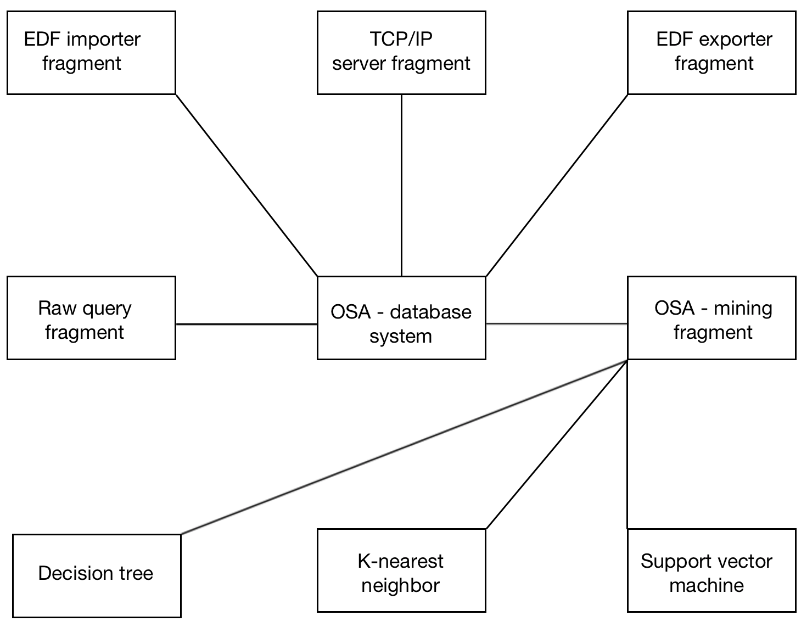
\includegraphics[width=1.0\textwidth]{Figures/OSADBSContext.png}
    \caption{The context of the OSA database system application}
    \label{fig:Figures/OSADBSContext}
\end{figure}
The first two and the last three requirements in Table \ref{tab:userrequirementAPP} are respectively corresponded to “what it must contain” and “what the database is to be used for” presented in the database modeling chapter. In other words, the database application needs to be implemented two wrappers that collect data from CESAR acquisition tool and EDF/EDF+ file formats, then the collected data can be used for analyzing, visualizing, or modifying. Since the mainly focus of the thesis are collecting data and data analysis, therefore visualizing and modifying are added as helper functions.\\
The first two user requirements illustrate that the system must support collecting samples from BITalino by using CESAR acquisition tool, and importing EDF/EDF+ data. As presented in Chapter 3, for collecting samples from CESAR acquisition tool, the system first establishes a TCP/IP connection to the tool, then the metadata and data packages are sent to the system. The structure of these packages are well documented, and have been discussed in Chapter 3. The user can also use multiple acquisition tools to collect sample, hence the application must support multiple connections as well. Since CESAR acquisition tool does not send the information of the clinic and patient, the information must be manually filled by the user before recording samples. CESAR acquisition tool provides data in real-time, therefore the system must operate with respect to the given non-functional requirements presented in Table \ref{tab:userrequirementAPP}. Likewise, for importing and exporting EDF/EDF+ files, the system must follow the structure of the EDF/EDF files which are also well discussed in Chapter 3. Since the files can be very large, the system must satisfy the non-functional requirements when importing and exporting.\\
As mentioned earlier, visualizing and modifying are not the main focus of the thesis. They are added to the database system application as helper functions to help the user have a better view on the collected data. Therefore, they are implemented as proof-of-concept and “enough for using”. For the analysis requirements, a raw query function is useful when analyzing the data. However, in term of security, this is quiet dangerous action. In the top 10 vulnerabilities, SQL injection stands on the top of the list\cite{OWASP}. In this case, the risk does not come from stealing of sensitive information, or compromising the database. It is dangerous if the researchers accidentally perform queries that can result the database system corrupted, such as deleting a column in a data table, drop a table, etc. Filter out vulnerable queries is a topic for researchers who are interested in database security. Hence, to filter out vulnerable queries is not in scope of the thesis. An assumption is made that the users have the knowledge on database system, and they do not perform any vulnerable queries. The system must also provide some of possible mining algorithms that are used for detecting OSA signal.
\section{System modeling}
As presented in Figure \ref{tab:userrequirementAPP}, the context of the OSA database system consists of importing, exporting and analyzing data. Data sources, in which the system collects data from, can be divided into two groups. Sources that connect to the database system via TCP/IP protocol are real-time sources. On the other hands, non-real-time sources are from EDF/EDF+ files. Data analysis are only performed on the stored data. Currently, the system does not support real-time analysis, since the goals of the system are collecting raw data for future analysis. That is, the collected data are used as the inputs for many different analysis algorithms than the possible mining methods presented in this thesis. However, real-time OSA data analysis is good to be considered, and an exciting topic for researchers who are interested in online analytical processing.\\
Subsection 5.2.1 presents real-time wrapper modeling, in which, some real-time attributes are taken into considered, and how the TCP/IP server fragment is modeled. Subsection 5.2.2 presents the modeling for non-real-time wrapper, in which EDF importer fragment and EDF exporter fragment are carefully modelled. Subsection 5.2.3 discusses training set, OSA pattern, and possible mining algorithms can be used for detecting OSA signal at abstract level.
\subsection{Real-time wrapper}
When choosing the appropriate real time sensor sources, several factors should be considered, such as the quality of signal, mobility, how many channels can it observe, which protocol it uses to send data sample, etc. The BITalino platform is chosen as sensor source after carefully considering the pros and cons of it in Chapter 3.\\
In terms of real-time data stream source, the system has to deal with data stream management problems. The thesis targets at a solution to store the OSA bio-signals, and it does not address data stream management system issues, where the queries need to be apply on the data stream. Instead, some general real time factors need to be seriously considered when designing the database system. These factors are arrival rate, timestamp, physical resource, one-time read data, data stale or imprecise, and unpredictable data arrival. When the incoming rate is high, it might be a problem to store all the data, because of the limitation of the mobile platform. Even on a stationary computer, storing data streams could be a problem and needs to be considered.\\
To choose a suitable solution for manage the arrival rate of the data stream, it is good to review and discuss how the data stream management system (DSMS) deal with real-time data stream problems. Due to the unboundedness of the data stream, it is essential to capture the stream into small slices which is called windows. To manage the data stream, DSMS uses window models, in which the models are based on the direction of movement of the endpoints, that are fixed window, sliding window, and landmark window. As the name of the window models, the fixed window has a fixed amount of samples or time interval. The sliding window contains the data from now up to a certain range in the past. The landmark window, on the other hand, contains the data from the beginning until now. The window size can be either physical/time-based or logical/count based. Figure \ref{fig:Figures/windows} presents an overview of the fixed window and sliding window.
\begin{figure}[ht]
    \centering
    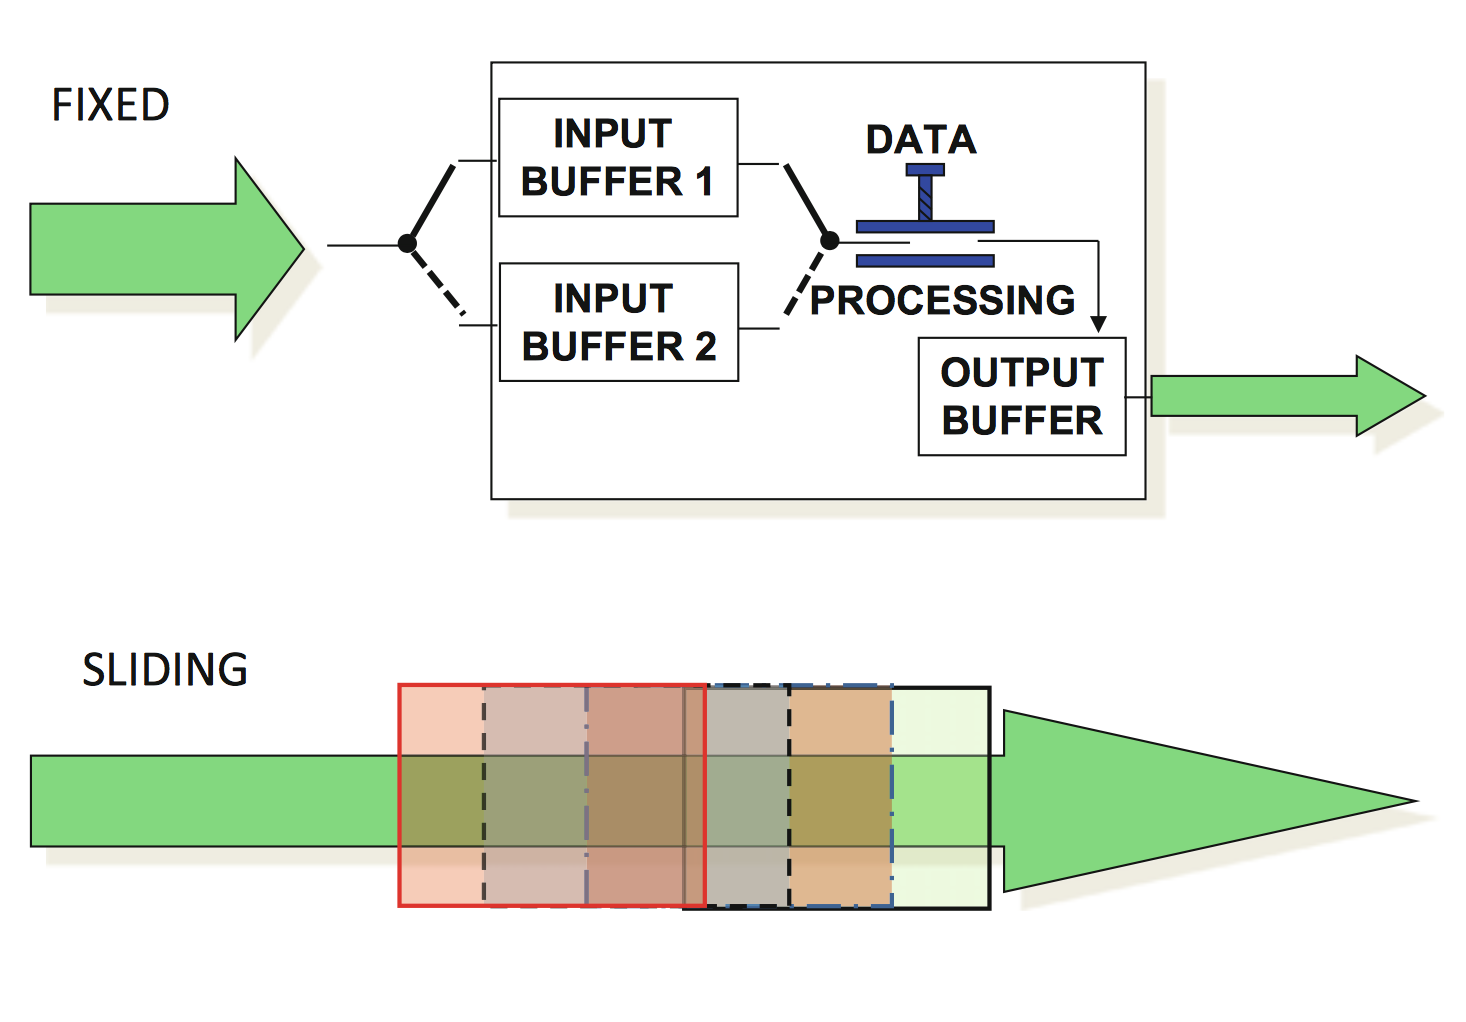
\includegraphics[width=0.6\textwidth]{Figures/WINDOWDSMS.png}
    \caption{Example of fixed and sliding windows \cite{DSMS_WINDOW}}
    \label{fig:Figures/windows}
\end{figure}
When a sample arrives, it is updated either immediately (eager processing) or when the window is full (lazy/batch processing).\\
Tasks of the system are to store the raw data samples as well as to display these samples to a graph view with respect to the users’ requirements. To ensure that the tasks are well performed, the system uses two buffers which functioned as windows in DSMS. It is to say, the first buffer is a fixed window, count based, and batch processing, that is used for collecting samples for the database. The second buffer is a sliding window, count (or time) based, eager processing, that is used for collecting samples for graphic view. By using these two buffer, the system ensures that the overhead of writing to database is minimized (by using batching processing), while the performance increases (by using eager processing).\\
If the order of the samples plays an important role for later analysis, the timestamp must be explicit (timestamp from data source). Otherwise, the implicit timestamp (system time) can be used. The CESAR acquisition tool provides the timestamp in each sample object. However, the timestamp is pre-converted and need to be handled before using for plot view. It is an overhead for converting timestamp for each sample. Moreover, the system uses local network for sending samples, and the assumption is made that the delay in network and order of the samples are acceptable. Therefore, the implicit timestamp is considered a better solution than the explicit timestamp with respect to system overhead, hence the performance is improved. A comparison between these timestamp is presented in Appendix XX.\\\\
\textbf{Server thread}\\
The collector of CESAR acquisition tool offers two methods for that the database application can collect data from it. The collector can either save data to a text file or send them to a given server IP and port address by using TCP/IP protocol. Since the database system application wants to have real-time data from BITalino, it must open a port to collect data. As presented in requirement section, the system must support multiple connections, because the user may use multiple sensor source to monitor the body. Therefore, multiple threads system must be implemented. Each thread manages one sensor source. The main thread therefore just waits for connections, creates and hands in necessary information to the new created thread, then starts the new thread. The main thread must have a way to manage the created threads for that the users can choose a source they want to interact with from the connected list. A Unified Modeling Language (UML) activity diagram is used for illustrating how the main thread works as presented in Figure \ref{fig:Figures/ServerActivity}. UML is a famous and widely used modeling language, however, a short explanation on the used annotations is needed to make the figures easier to understand. In UML activity diagram, a filled circles indicates the start of a process. Activities are presented by rectangles with round corners. Arrows present the flow of work between activities. Annotations on the arrow indicate the condition when the work flow is taken. A filled circle inside another circle indicates the end of the process.\\
\begin{figure}[ht]
    \centering
    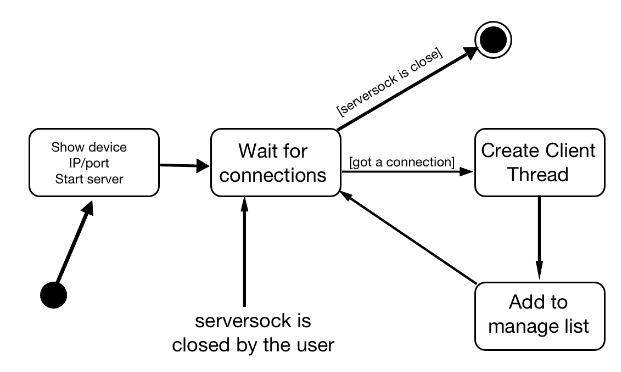
\includegraphics[width=1.0\textwidth]{Figures/ServerActivity.png}
    \caption{Process model of server thread}
    \label{fig:Figures/ServerActivity}
\end{figure}
\textbf{Client thread}\\
Most of the jobs of the wrapper are handled in the client thread. Once a client thread is created, it waits for arrival data, then pushes to database or adds to graphical view if these actions are flagged. Data packages from CESAR acquisition tool are well discussed in Chapter 3, in which a metadata package is sent first to identify the sensor source, then the source keeps sending its data via the connection between the database system application and the acquisition tool. As explained in the real-time characteristics, the client thread must share two buffers with the other threads. The first buffer is used for storing samples to the database, and the second buffer is used for showing samples on a graphic view. However, these buffers are initialized only if the corresponded flags are flagged. That is, arrival samples are thrown if the users do not want to store or visualize them. Figure \ref{fig:Figures/ClientThreadAc} presents a possible implementation of the client thread by using a UML activity diagram.
\begin{figure}[ht]
    \centering
    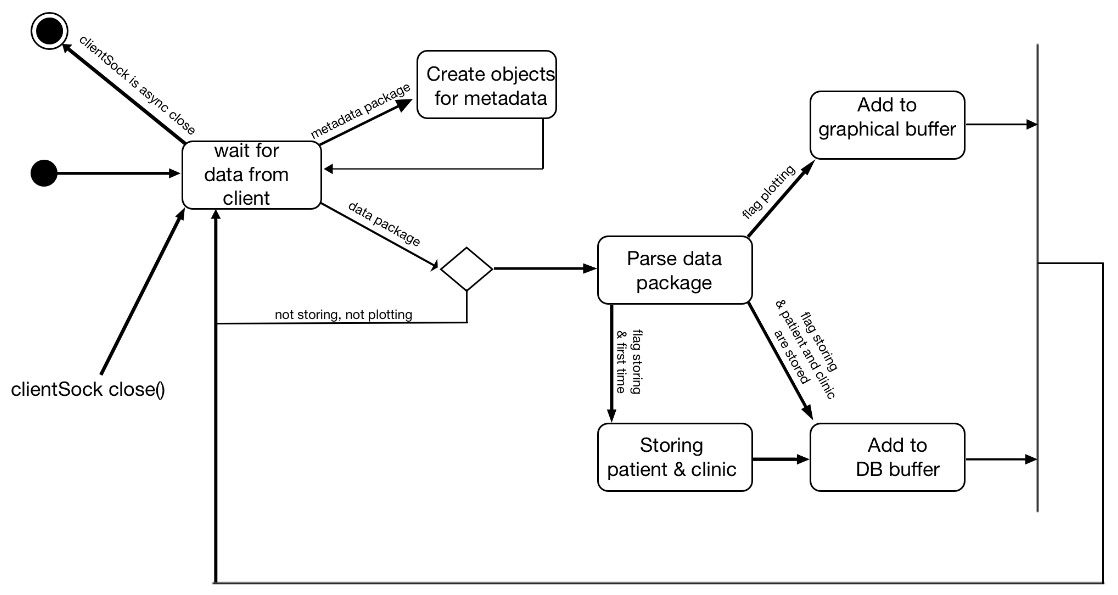
\includegraphics[width=1.0\textwidth]{Figures/ClientThreadAc.png}
    \caption{Process model of client thread}
    \label{fig:Figures/ClientThreadAc}
\end{figure}
As illustrated in the requirements, the system must be reliable and have a good performance. That is, no samples data are lost under recording, and the visualization must not be frozen. To satisfy these requirements, two different buffer management methods are used. A buffer, which is used for storing samples, maintains a list of fixed number of samples (it is to say, a record fragment), and a thread. The thread takes a full record fragment to store into the database, or waits for available record fragments if the list is empty. Since SQLite can perform about 50,000\cite{SQLITEORG_INSERT} insert statements per second, while the maximum number of samples BITalino can delivery is 1000 samples per second (1000Hz), the algorithm for this buffer is therefore satisfied the non-functional requirement (reliable). The second buffer can be implemented by using the algorithm from Producer and Consumer problem, in which the client thread is the producer, and a thread that update the graphic view is the consumer. However, this buffer is used as a sliding window, therefore a simpler solution can be used. That is, each time client thread adds a sample to a buffer list, it removes the oldest sample if the buffer is full. After that, a graphic view thread is notified to refresh the plot view.\\
Figure \ref{fig:Figures/ThreadsDBPlot} presents how the sever thread, client thread, database, and graphic view connect to each other’s.
\begin{figure}[ht]
    \centering
    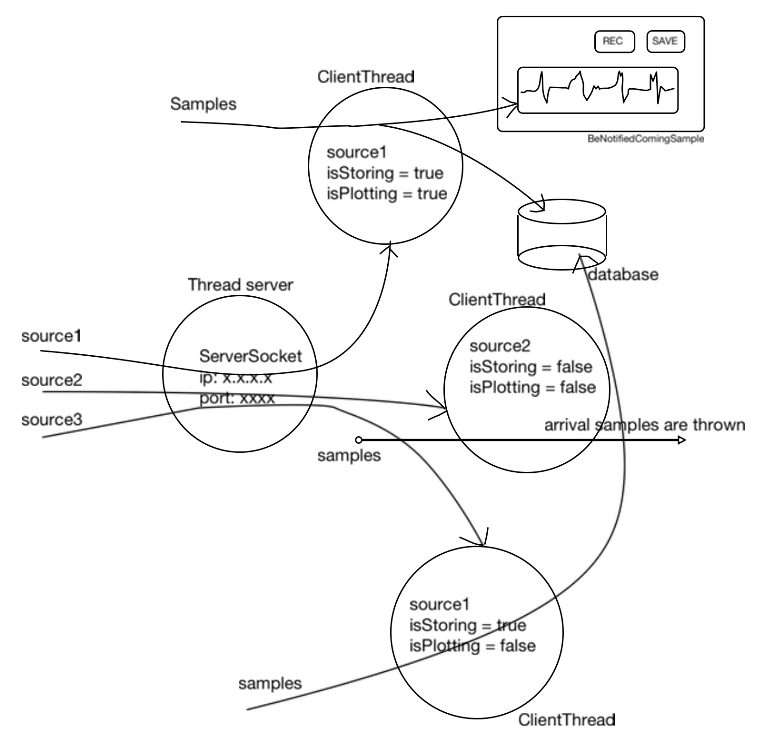
\includegraphics[width=1.0\textwidth]{Figures/ThreadsDBPlot.png}
    \caption{High level design of real-time wrapper}
    \label{fig:Figures/ThreadsDBPlot}
\end{figure}
\subsection{Non real-time wrapper}
Diverse data sources are essential in research. Using multiple sources of data in research often produces more accurate results and more objective values than using a single data source. There are many trustworthy sources that can be used for OSA data analysis. One of the sources that is chosen in this thesis are the Physionet sensor databases, which have been described in Section 3.1.2. The other non-real time source that the system collects data from, is NOX-T3 sensor source system. Theoretically, this source can be used as a real time sensor source. Although Nox-medical has an Android application, which is only support NOX-A1-PSG at the time of this writing, to collect samples from their devices, the NOX-T3 device neither provide any API for mobile platform, nor any documents that describe how to collect samples from the device as BITalino does. As mentioned earlier, it is very difficult to manage diverse sources when they have their own format. Fortunately, the problem is solved by using an EDF or an EDF+ file format to share data between source owners. The formats are fully described in Section 3.2.2 with respect to why they are introduced, what information these file contain, and how to use them. Therefore, the system is designed in the way that is opened for all of the sensor sources, as long as these sources can export their data to an EDF or EDF+ file format. In other words, the system only accepts source files in EDF form.\\
An EDF file can be very large, and can excess the main memory size. Hence, to satisfy the performance and robustness, the system should neither keep all the data in memory, nor call the database insert function for each sample. The problem could be solved by using the idea from real time sensor source. In other words, the system uses the concept of a window model, lazy update (batch processing) to solve the memory problem with the non-real time source.\\
Physionet databases and NOX-T3 sensor source can be used as non-real-time sources, because both of them provide a function to export their bio-signal data to EDF. “mit2edf” is a function from physiotools provided by Physionet. This function is used for converting between EDF and WFDB-compatible formats. NOX-T3 provides a graphic, step by step, and user friendly way to export their data to EDF.
\subsubsection{EDF importer}
As introduced in Chapter 3, EDF is one of the standardized data formats for bio-signals that used for storing and exchanging multichannel biological and physical signals. There is many tools and open source codes which can be used for reading a EDF file. Different tools have different goals when reading the EDF file. Most of them parse the samples to a graphical view and an annotations list, the others try to convert samples into text files that contain information for each channel and the record. EDF browser and EDF library\cite{EDFLIB} are one of the most famous used tools to view and parse EDF files. The performance of the tools is quite good since they are written in C code. Another open source tool that can be used for parsing EDF files to text files is Java-parser for EDF format\cite{EDF4J}. As the tool named, it is written in Java code, hence, the performance when parsing EDF file is poorer compared with EDF library. Since EDF/EDF+ file formats are well documented, it is easy to write a parsing tool. As discussed, different tools have different purposes when parsing EDF files. Since the one of the main goals of EDF file format is used for exchanging biological data, the EDF files need to be parsed into the received system data structure. Many parsers try to load the whole EDF file into main memory before converting. As discussed, the EDF file can be extremely large, the parsers therefore crash; Java-parser for EDF format is one them.\\
There is no need to “reinventing the wheel” rather using them in a smart way. Since in the designed database system, each bio-object is stored in a separate table. Therefore, the EDF importer can use the functions in an EDF library to read the EDF files. The information, which are read from EDF, are stored into the corresponded tables. In case the used library tries to read the whole EDF file into memory, an optimization, which is multiphase read, need to be used. Figure \ref{fig:Figures/EDFImporter} presents a UML activity diagram which explains how a EDF file can be read into the database without memory problem.
\begin{figure}[ht]
    \centering
    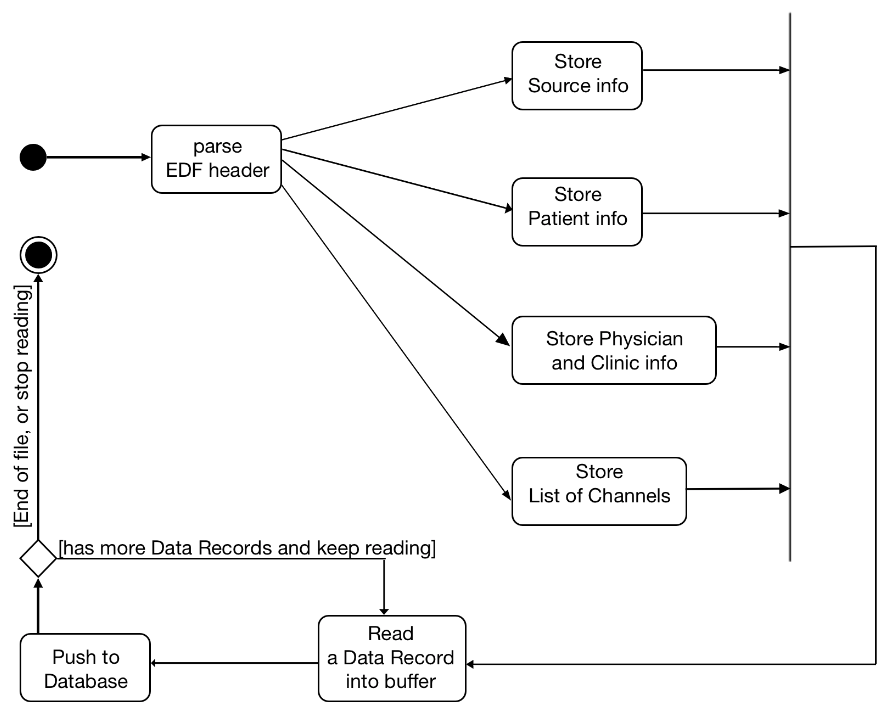
\includegraphics[width=1.0\textwidth]{Figures/EDFImporter.png}
    \caption{Process model of EDF importer}
    \label{fig:Figures/EDFImporter}
\end{figure}
\subsubsection{EDF exporter}
Sharing data is essential in researching. Therefore, the system must export its data into a standardized data formats for bio-signals, a EDF file. On the other hands, the system targets to be implemented on a mobile platform, where resources are very limited. Exporting data and saving it in external storage places is vital to satisfy non-functional requirements, where the collected data must not be lost when the storage capability of the mobile devices exceed. There is no need to export the whole source of data to a EDF file, some of channels or samples are exported for special needs. For example, there is a project, in which researchers or physicians need only samples from ECG channel, it does not make sense if the EDF file contains samples for the other non-relevant channels. Furthermore, if a project needs to analyze all samples which collected on nighttime, the added daytime samples are waste of not only the storage, but also time to parse the EDF file when using. Therefore, the system must let the users choose which channels and periods they want to export. As discussed in the non-functional requirements for EDF importer and exporter, the information of the patient must follow the protection of personal data law. That is, the patient must be exported as anonymous, otherwise there must be an agreement of the patient. Figure \ref{fig:Figures/EDFExporter} is a UML activity diagram that illustrate how data are exported into a EDF file.
\begin{figure}[ht]
    \centering
    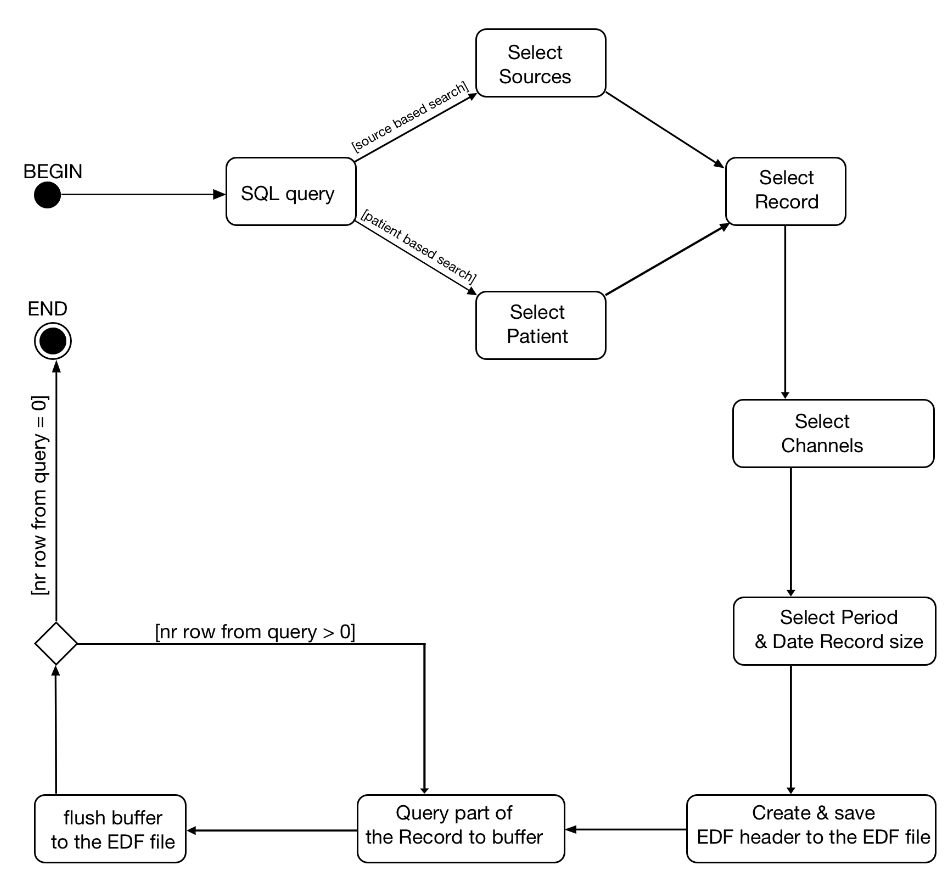
\includegraphics[width=1.0\textwidth]{Figures/EDFExporter.png}
    \caption{Process model of EDF exporter}
    \label{fig:Figures/EDFExporter}
\end{figure}
\section{Android specific design and implementation}
\subsection{Graphical user interface}
\subsection{CESAR wrapper}
\subsection{EDF wrapper}
\subsection{Mining}
\subsubsection{Workload generator}
\subsubsection{OSA pattern and trained sets}
\subsubsection{Possible mining algorithms}
\textbf{Decision tree}\\
\textbf{K-nearest neighbor}\\
\textbf{Support Vector Machine}\\
\textbf{Artificial Neural Network}